\documentclass[11pt]{utalcaDoc}
\usepackage{alltt}
\usepackage{underscore}
\usepackage[utf8]{inputenc}
\usepackage[activeacute,spanish]{babel}
\usepackage{verbatim}
\usepackage[pdftex]{graphicx}
\usepackage{ae}
\usepackage{amsmath}
\usepackage{amsfonts}
\usepackage{pdflscape}
\usepackage{inconsolata}
\usepackage{url}
\usepackage{hyperref}
\usepackage{listings}
% \usepackage{placeins}
\usepackage[section]{placeins}
\usepackage[stable]{footmisc}


\title{{\bf Seguridad Informática}\\ Tarea 2}

\author{Erik Regla\\ eregla09@alumnos.utalca.cl}
\date{\today}
\lstset{language=SH, 
		basicstyle=\ttfamily\tiny, 
		showspaces=false, 
		numbers=left, 
		breaklines=true,
		frame=shadowbox
		}

\begin{document}

\maketitle

\section{Enunciado}
Deberá entregar un informe sobre la técnica denominada Esteganografía, donde
deberá definir que es e identificar en cual o cuales de las fases de un ataque
informático se utiliza. Además deberá entregar un ejemplo concreto de su
utilización.

\section{Desarrollo}

\subsection{ Definición de esteganografía }
La esteganografía se define como el encapsulado de información utilizando otro medio como portador. Uno de los ejemplos más simples es el de la utilización de tinta invisible reactiva a UV (popular en los años 90). La diferencia en la coloración del papel de la tinta invisible es casi inperceptible para el ojo humano, sin embargo, al ser expuesto el papel a una fuente de radiación UV, esta brilla con tonos fosforecentes dejando visible el mensaje oculto en el medio (figura \ref{INVISIBLE_INK}).

\begin{figure}[]
    \centering
    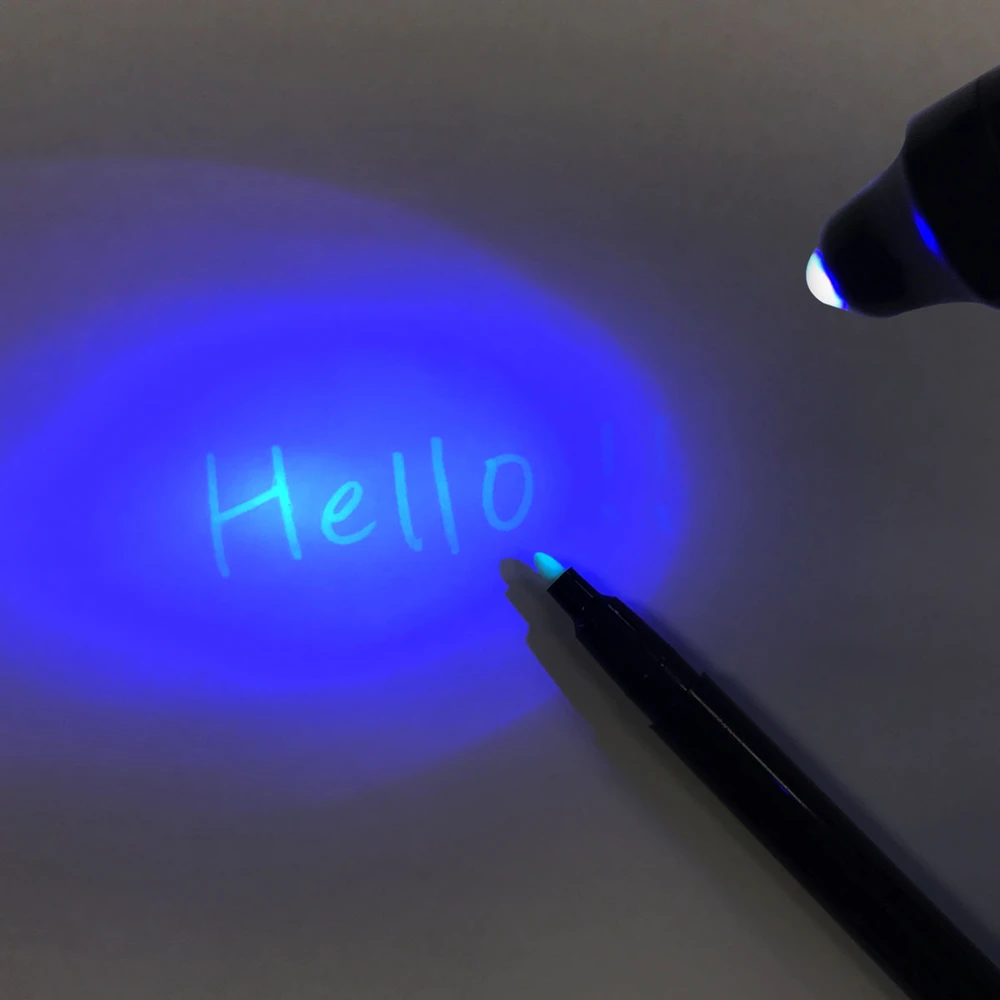
\includegraphics[width=0.5\textwidth]{invisibleink.png}
    \caption{Ejemplo de uso de tinta invisible}
    \label{INVISIBLE_INK}
\end{figure}


\subsection{ Utilización en un ataque informático }
Esteganografía como técnica puede ser utilizada para ocultar información en archivos que admitan el concepto de ``perdida de compresión''\footnote{https://en.wikipedia.org/wiki/Lossy_compression}. Si bien esta puede ser utilizada sobre archivos que no admitan pérdida, si detección es mucho mas simple. Casos como este son las muestras de puntos que dejan las impresoras laser, las cuales permiten identificar que impresora imprimió un documento y su firma de tiempo. Estas no son perceptibles por un ojo humano, pero si son fácilmente identificables por una máquina (figura \ref{PRINTER}).

\begin{figure}[]
    \centering
    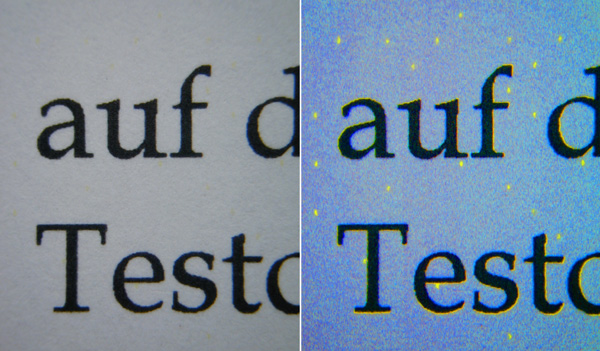
\includegraphics[width=0.5\textwidth]{printer.png}
    \caption{Puntos amarillos de las impresoras}
    \label{PRINTER}
\end{figure}

Ejemplos de este tipo de archivos son archivos de imágenes en formato jpg, audio en formato ogg o mp3. Esta técnica no está limitada solo al uso de estos formatos, pero son los más simples de encontrar.

% Para la definición de en que etapas se utiliza esta técnica vamos a abandonar la definición de 5 etapas de un ataque informático ya que como es sabido tanto las métricas utilizadas como las mismas certificaciones ofrecidas por el EC-Council tienen nula validez cuando se trata de IT-Sec. Debido a esto, vamos a utilizar el modelo de Cyber Kill-Chain (CKC) de Lockheed Martin\footnote{https://www.lockheedmartin.com/en-us/capabilities/cyber/cyber-kill-chain.html} el cual al estar enfocado en IT-Sec y no Info-Sec, deglosa en profundidad como son utilizados los artefactos durante un ataque en la práctica y no conceptualmente.
%% quizás no debería continuar esto para prevenir ajís en el hoyo

Durante la etapa de reconocimiento puede ser utilizado para obtener información por medio de la propagación de medios y firmas (por ejemplo, trazar los usuarios que tuvieron contacto con un contenido), ocultar información de identidades u otra necesaria para esta. Durante la etapa de adquisición de acceso puede ser utilizada para transportar datos o cargas a un equipo destino para su posterior ejecución, de ahí en adelante su uso permite la mantención de acceso. Debido a esto, se puede decir que esta técnica primariamente considera tres de las cinco fases de un ataque, sin embargo, transitivamente puede extenderse a ocultar rastros (ya que por lo general el proceso de estenografía es ejecutado de manera ortogonal) y a la etapa de exploración debido a las mismas características del escaneo por su uso en pentesting físico.\footnote{https://publications.computer.org/computer-magazine/2018/11/15/how-steganography-works/}


\subsection{ Ejemplo de utilización }

Uno de los ejemplos más simples de visualizar es el ocultar cargas ejecutables dentro de un archivo de uso común, como por ejemplo una imagen digital\footnote{https://securelist.com/steganography-in-contemporary-cyberattacks/79276/}.


\lstinputlisting[language=Bash]{script.sh}

\end{document}